\documentclass[main.tex]{subfiles}
\begin{document}

\title{
    \textbf{Algorytmy ewolucyjne i metaheurystyki}\\
    \begin{large}
        Sprawozdanie 4
    \end{large}
}

\author{
    Górka Bartosz\\
  \texttt{127228}
  \and
  Zimniak Kajetan\\
  \texttt{127229}
}

\date{}

\maketitle

\section{Opis etapu projektu}
Celem kolejnego etapu projektu była implementacja dwóch algorytmów przeszukiwania lokalnego. Pierwszym z nich był \texttt{Multiple Start Local Search}. Został on uruchomiony 10-cio krotnie, każdorazowo realizujący 100 operacji przeszukiwania lokalnego ze zrandomizowanym przydziałem punktów do grup.

Drugi algorytm to \texttt{Iterated Local Search}, który został przygotowany w trzech wersjach. Pierwsza realizuje małą perturbację polegającą na przeniesieniu 2\% punktów pomiędzy grupami w sposób zrandomizowany. Dwie pozostałe realizują dużą perturbację z przeniesieniem 30\% punktów. W fazie \texttt{Destroy} zostają wytypowane i usunięte punkty. Jedna z wersji realizuje to w sposób losowy, druga natomiast wybiera najbardziej oddalone od reszty grupy punkty. Kolejną fazą jest \texttt{Repair} z przydziałem punktu do grupy, dla której najmniej pogarsza wartość funkcji celu.

Liczba grup pozostała bez zmian na poziomie 20. Podobnie jak w poprzednich etapach, funkcja celu została zdefiniowana jako \texttt{minimalizacja średniej odległości wszystkich par obiektów umieszczonych w ramach tej samej grupy}.

W rozdziale \ref{section:pseudokody} zaprezentowano pseudokody przygotowanych rozszerzeń algorytmu, natomiast w rozdziale\leavevmode\nobreak\ \ref{section:wyniki} wyniki działania. Ostatni rozdział dotyczy wizualizacji najlepszych uzyskanych rozwiązań.

\section{Pseudokody}
\label{section:pseudokody}
\subsection{Multiple Start Local Search}
\begin{verbatim}
W pętli wykonaj iterację aż osiągniesz limit iteracji lokalnego przeszukiwania {
    Zainicjalizuj losowy przydział punktów do grup

    W zależności od parametru metody, wykonaj przeszukiwanie lokalne z wykorzystaniem
    algorytmu Greedy bądź Steepest

    Jeżeli osiągnięto lepsze rozwiązanie niż do tej pory najlepsze {
        Zapisz wartość funkcji celu
        Zapisz uzyskany przydział punktów do grup
    }
}
\end{verbatim}
W naszym przypadku procedura opisana wyżej powtarzana jest 10-cio krotnie, za każdym razem zapamiętujemy uzyskany wynik i przydział punktów do grup.

\subsection{Iterated Local Search}
\begin{verbatim}
Wyznacz liczbę punktów do przeniesienia w zależności od użytej perturbacji
Wykonuj dopóki nie przekroczono limitu czasu wykonania {
    Dokonaj perturbacji rozwiązania startowego

    Z wykorzystaniem algorytmu Steepest wyznacz optimum lokalne

    Jeżeli wyznaczone rozwiązanie jest lepsze niż dotychczas najlepsze {
        Zapamiętaj wartość rozwiązania jako nowe najlepsze
        Za rozwiązanie startowe przypisz uzyskane rozwiązanie
    }
}
\end{verbatim}
Algorytm wykorzystuje metodę perturbacji. Jej dokładna realizacja została przedstawiona w kolejnych podrozdziałach, aby nie powielać opisu.

\subsection{Mała perturbacja}
\begin{verbatim}
Wykonuj aż do przeniesienia zakładanej liczby punktów {
    Wyznacz losowo grupę z której przenieść punkt
    Wyznacz grupę docelową inną niż startowa

    Wybierz punkt z grupy

    Przenieś go pomiędzy grupami
}
\end{verbatim}

\subsection{Duża perturbacja losowa}
\begin{verbatim}
W fazie Destroy usuń zakładaną liczbę punktów z grup (wybierz punkty losowo)

Dla każdego usuniętego punktu {
    Wyznacz grupę dla której najmniej pogarsza wartość funkcji celu

    Dodaj punkt do wyznaczonej grupy
}
\end{verbatim}

\subsection{Duża perturbacja heurystyczna}
\begin{verbatim}
Wyznacz sumę odległości każdego punktu od innych w ramach tej samej grupy
Posortuj listę zgodnie z malejącą sumą odległości

W fazie Destroy usuń zakładaną liczbę punktów z grup
iterując na przygotowanej liście punktów

Dla każdego usuniętego punktu {
    Wyznacz grupę dla której najmniej pogarsza wartość funkcji celu

    Dodaj punkt do wyznaczonej grupy
}
\end{verbatim}

\section{Wyniki eksperymentów obliczeniowych}
\label{section:wyniki}

W tabeli \ref{table:wyniki} zaprezentowano wyniki eksperymentów obliczeniowych. Dokonano $100$ powtórzeń obliczeń. Za każdym razem algorytmy zostały uruchomione dla rozwiązań startowych zbudowanych z wykorzystaniem algorytmu naiwnego.
\begin{table}[H]
\centering
\caption{Wyniki eksperymentów obliczeniowych}
\label{table:wyniki}
\resizebox{\textwidth}{!}{%
\begin{tabular}{|c|r|r|r|r|}
\hline
\textbf{Cecha} &                                                        \multicolumn{1}{c|}{\textbf{MSLS}} & \multicolumn{1}{c|}{\textbf{ILS small perturbation}} & \multicolumn{1}{c|}{\textbf{ILS big perturbation}} &
\multicolumn{1}{c|}{\textbf{ILS big perturbation heuristic}} 

                                       \\ \hline
\textbf{\begin{tabular}[c]{@{}c@{}}Wartość maksymalna\\funkcji celu\end{tabular}}
&   26.39
&   26.68
&   26.57
&   26.57\\ \hline
\textbf{\begin{tabular}[c]{@{}c@{}}Wartość średnia\\funkcji celu\end{tabular}}
&   26.37
&   26.68
&   26.39
&   26.57                                                 \\ \hline
\textbf{\begin{tabular}[c]{@{}c@{}}Wartość minimalna\\funkcji celu\end{tabular}}
&   26.37
&   26.68
&   26.39
&   26.57                                                 \\ \hline
\textbf{\begin{tabular}[c]{@{}c@{}}Wartość minimalna\\czasu obliczeń {[}sec{]}\end{tabular}}
&   73.79
&   798.87
&   799.04
&   799.00                                               \\ \hline
\textbf{\begin{tabular}[c]{@{}c@{}}Wartość maksymalna\\czasu obliczeń {[}sec{]}\end{tabular}}
&   111.97
&   798.87
&   799.04
&   799.00                                               \\ \hline
\textbf{\begin{tabular}[c]{@{}c@{}}Wartość średnia\\czasu obliczeń {[}sec{]}\end{tabular}}
&   79.88
&   798.87
&   799.04
&   799.00                                                \\ \hline
\end{tabular}%
}
\end{table}
Algorytm MSLS osiągał średnio najlepsze wyniki. Niewiele gorzej sprawdził się ILS z dużymi perturbacjami. Zgodnie z oczekiwaniami wprowadzanie niewielkich zmian w przydziale do grup nie wystarczało, by znacząco oddalić się od minimów lokalnych i końcowo algorytm z małymi perturbacjami nie osiągał wysokich wyników. W porównaniu z poprzednimi testowanymi algorytmami, stworzone w ramach czwartego etapu projektu działają o wiele dłużej. Spowodowane jest to oczywiście ich charakterystyką, tym, że złożone są właściwie z wielokrotnych powtórzeń lokalnego przeszukiwania.

\section{Wizualizacja najlepszych rozwiązań}
Podobnie jak w poprzednich etapach projektu, również w tym zastosowano wizualizację najlepszych rozwiązań na trzy sposoby. Pierwszy z nich to zaprezentowanie samych grup punktów, bez jakichkolwiek powiązań. Drugim sposobem jest prezentacja zgodna z funkcją celu, czyli zaprezentowanie powiązań pomiędzy punktami w ramach grupy. Ostatni sposób wykorzystuje minimalne drzewo rozpinające, które w przejrzysty sposób prezentuje przydział punktów do grup.

\begin{figure}[H]
     \begin{center}
        \subfigure{
            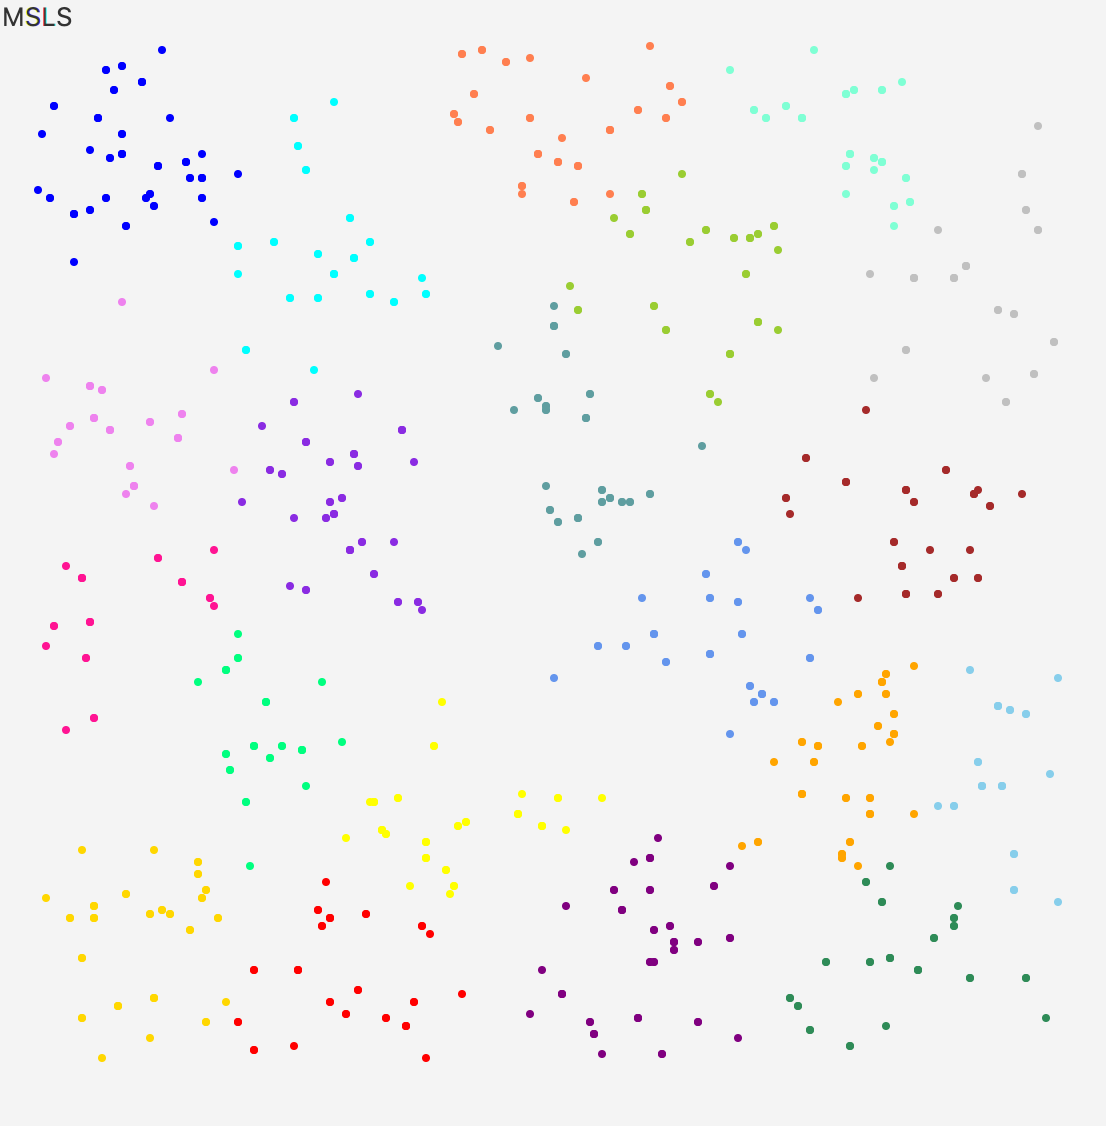
\includegraphics[width=0.45\textwidth]{sprawozdanie_4/msls.PNG}
        }
        \subfigure{
           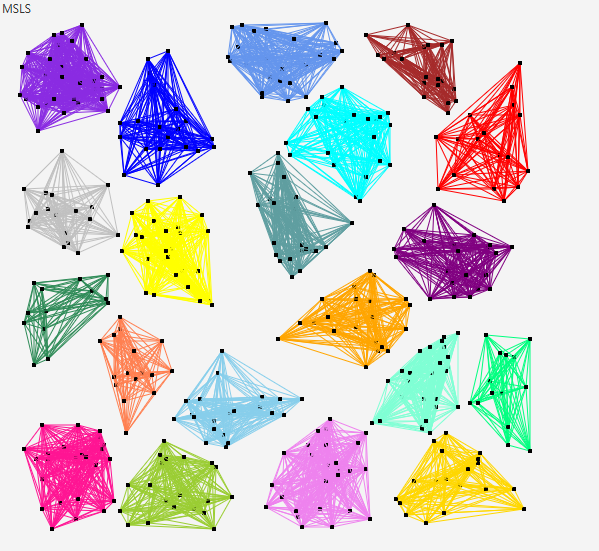
\includegraphics[width=0.45\textwidth]{sprawozdanie_4/msls_groups.PNG}
        }\\
        \subfigure{
            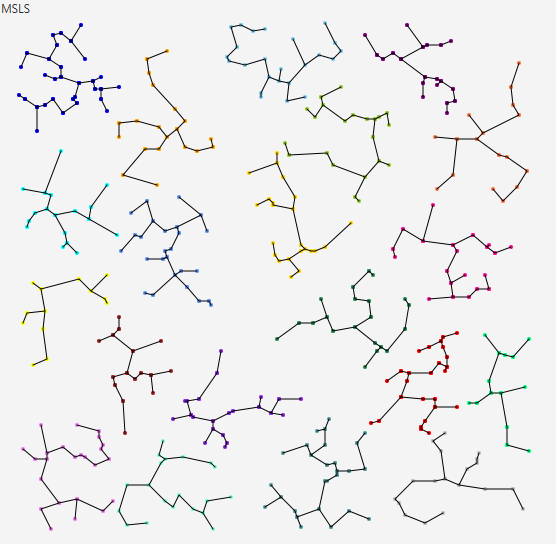
\includegraphics[width=0.45\textwidth]{sprawozdanie_4/msls_mst.PNG}
        }
    \end{center}
    \caption{MSLS}
\end{figure}

\begin{figure}[H]
     \begin{center}
        \subfigure{
            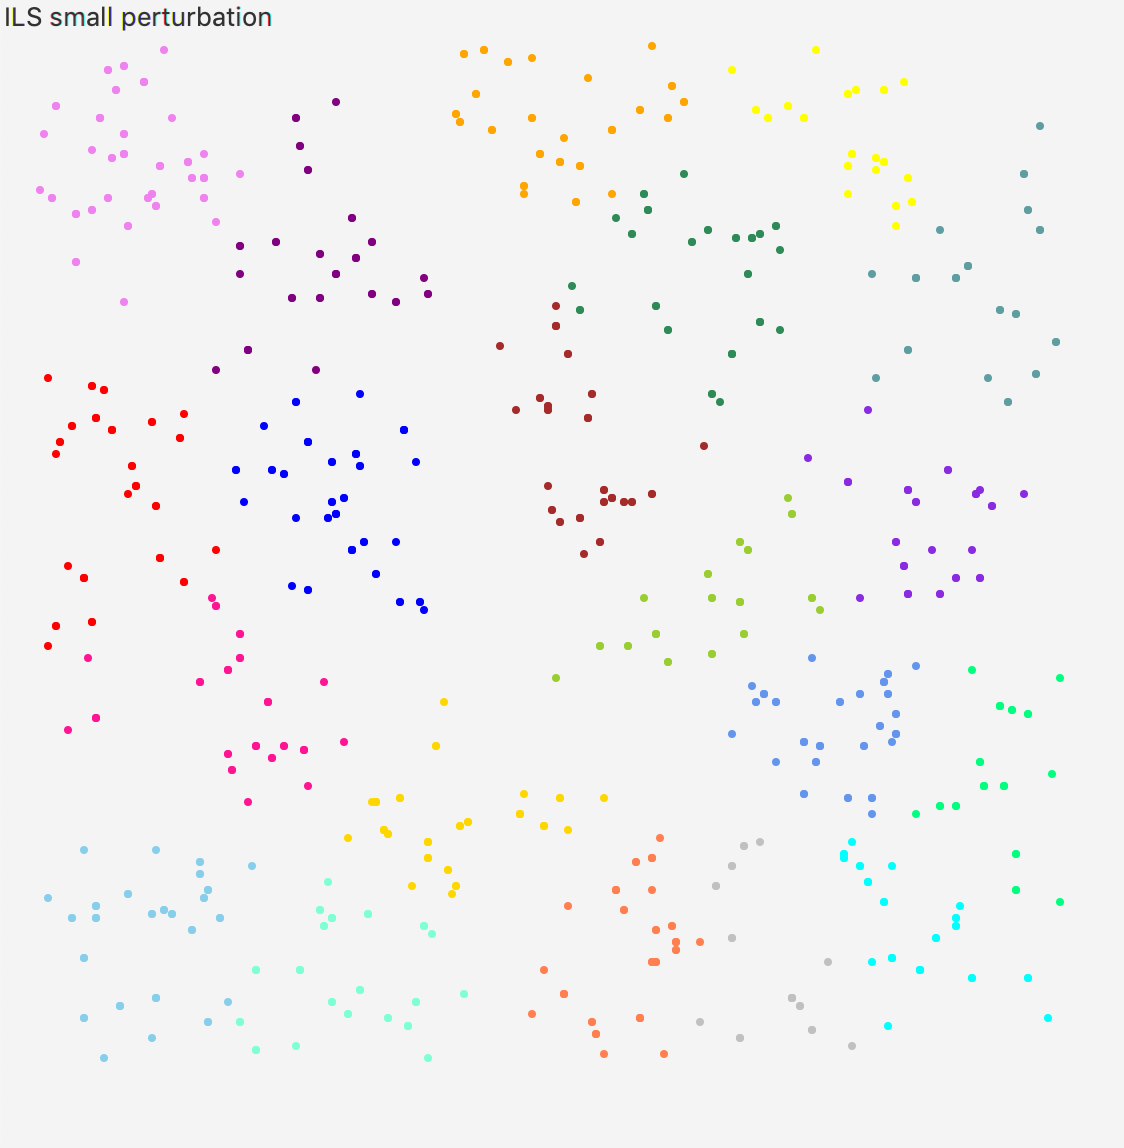
\includegraphics[width=0.45\textwidth]{sprawozdanie_4/ils_small.PNG}
        }
        \subfigure{
           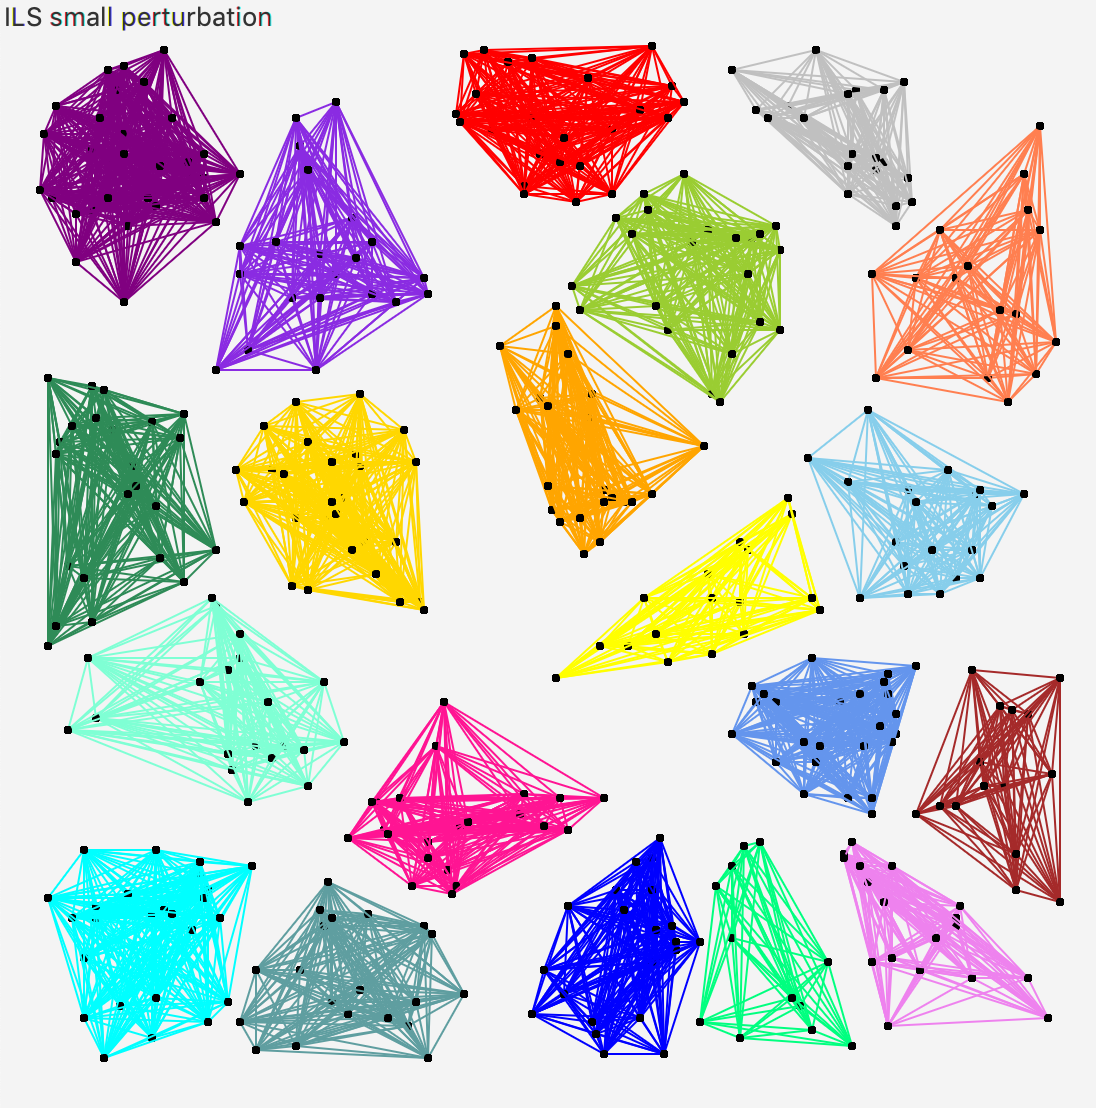
\includegraphics[width=0.45\textwidth]{sprawozdanie_4/ils_small_groups.PNG}
        }\\
        \subfigure{
            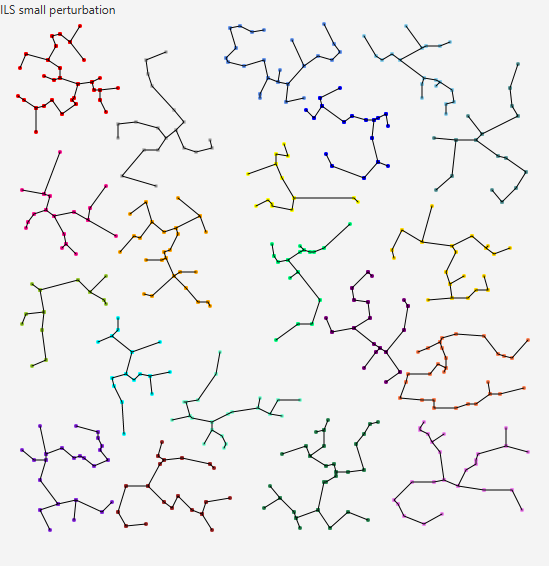
\includegraphics[width=0.45\textwidth]{sprawozdanie_4/ils_small_mst.PNG}
        }
    \end{center}
    \caption{ILS small perturbation}
\end{figure}

\begin{figure}[H]
     \begin{center}
        \subfigure{
            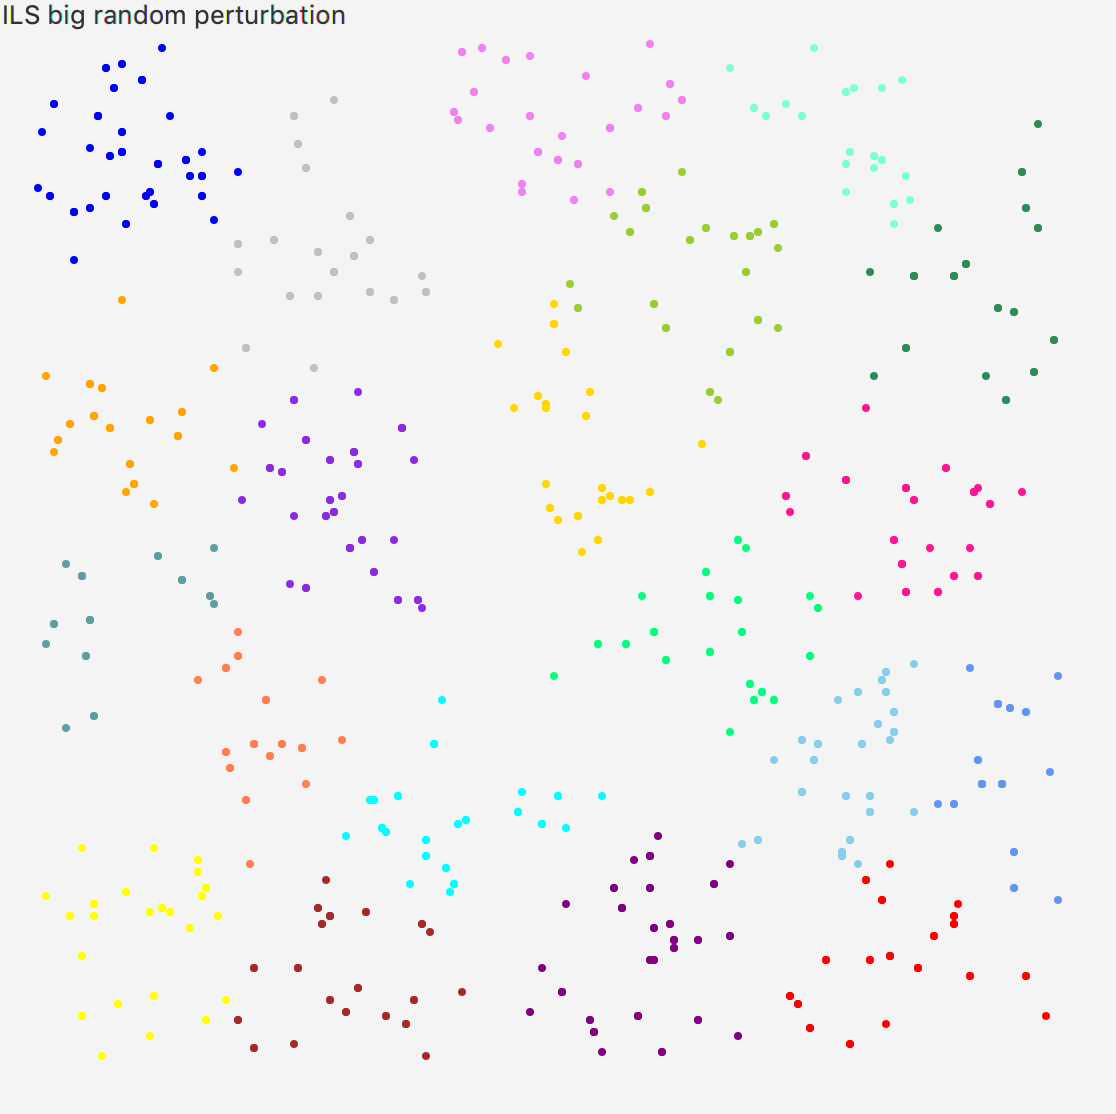
\includegraphics[width=0.45\textwidth]{sprawozdanie_4/ils_big.PNG}
        }
        \subfigure{
           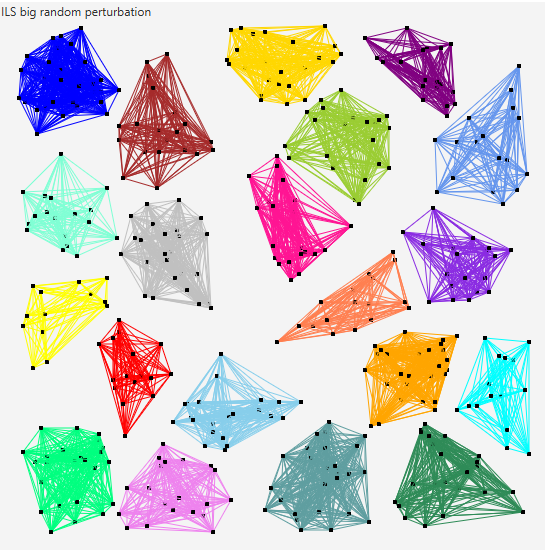
\includegraphics[width=0.45\textwidth]{sprawozdanie_4/ils_big_groups.PNG}
        }\\
        \subfigure{
            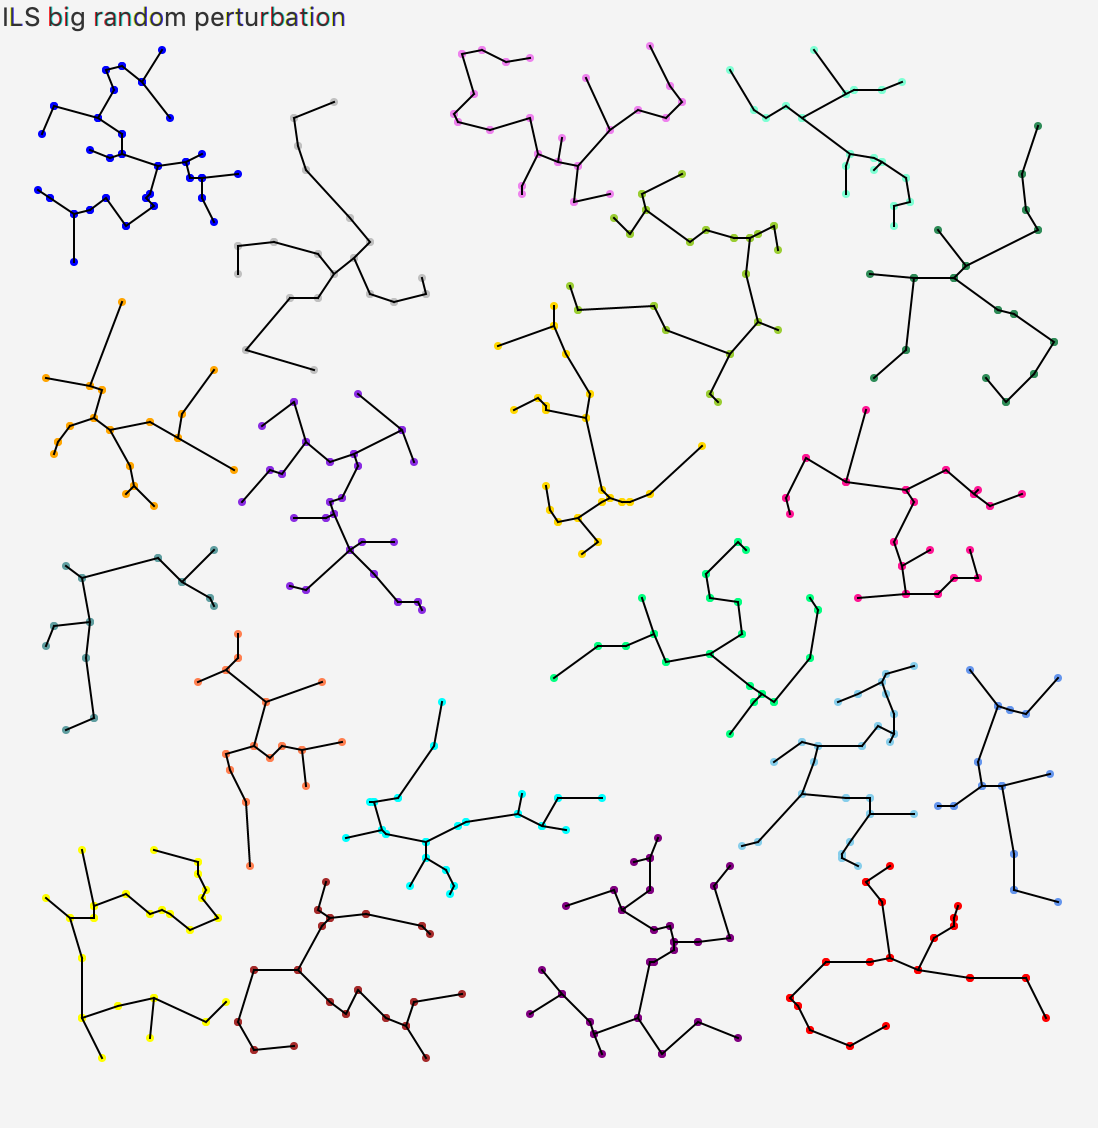
\includegraphics[width=0.45\textwidth]{sprawozdanie_4/ils_big_mst.PNG}
        }
    \end{center}
    \caption{ILS big perturbation}
\end{figure}

\begin{figure}[H]
     \begin{center}
        \subfigure{
            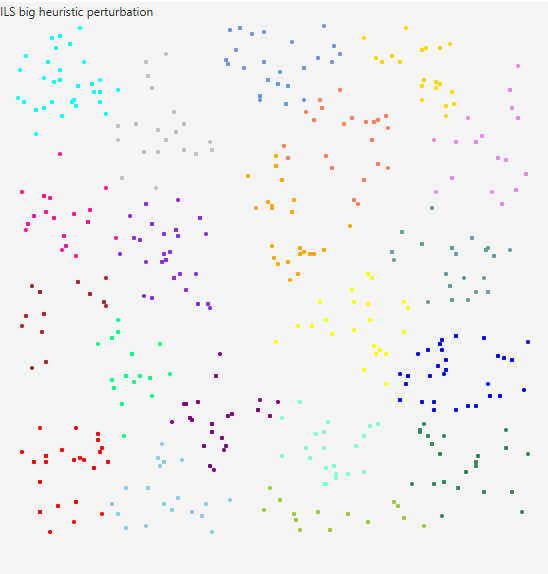
\includegraphics[width=0.45\textwidth]{sprawozdanie_4/ils_heuristic.PNG}
        }
        \subfigure{
           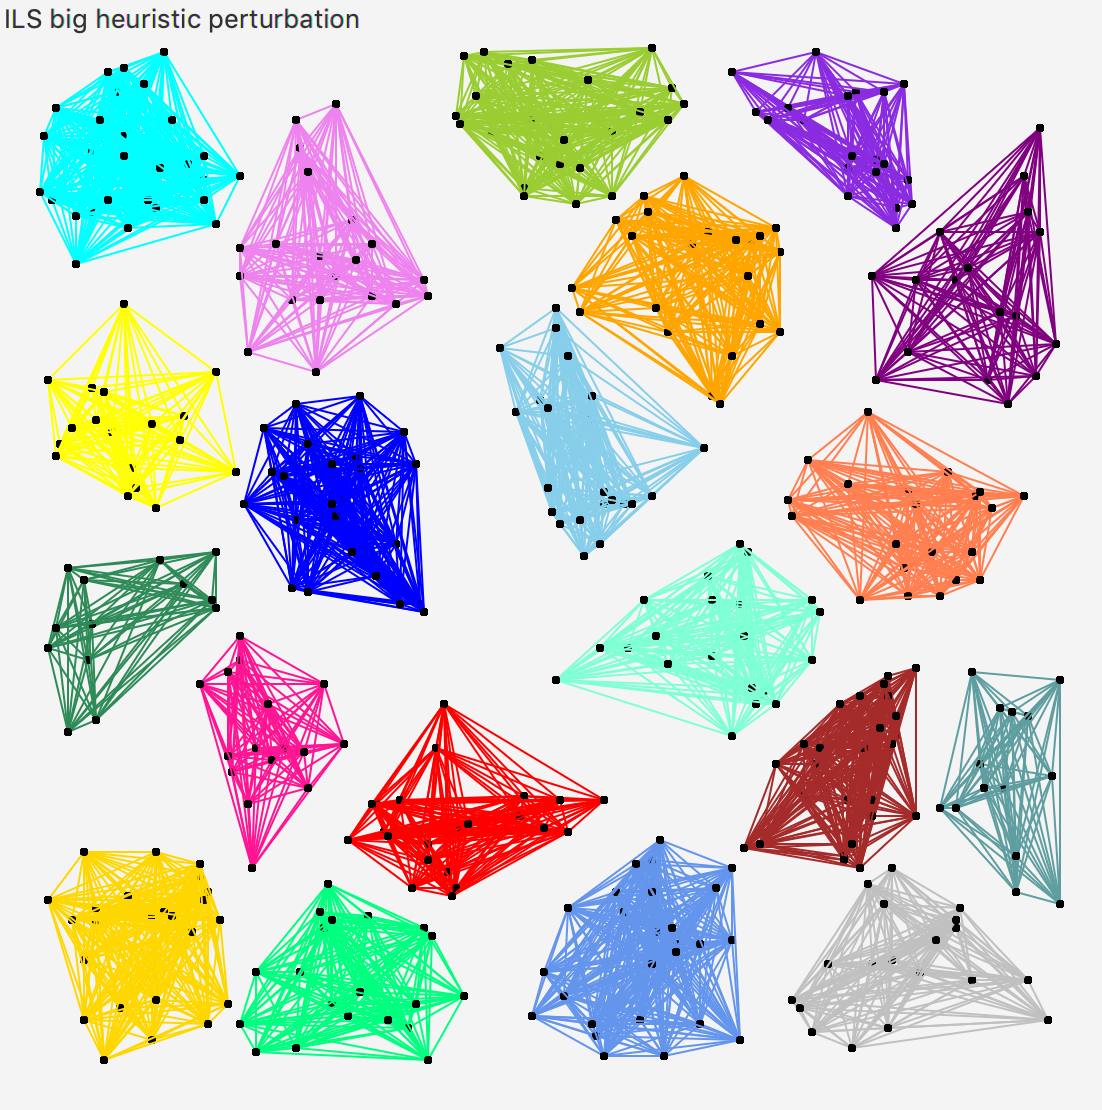
\includegraphics[width=0.45\textwidth]{sprawozdanie_4/ils_heuristic_groups.PNG}
        }\\
        \subfigure{
            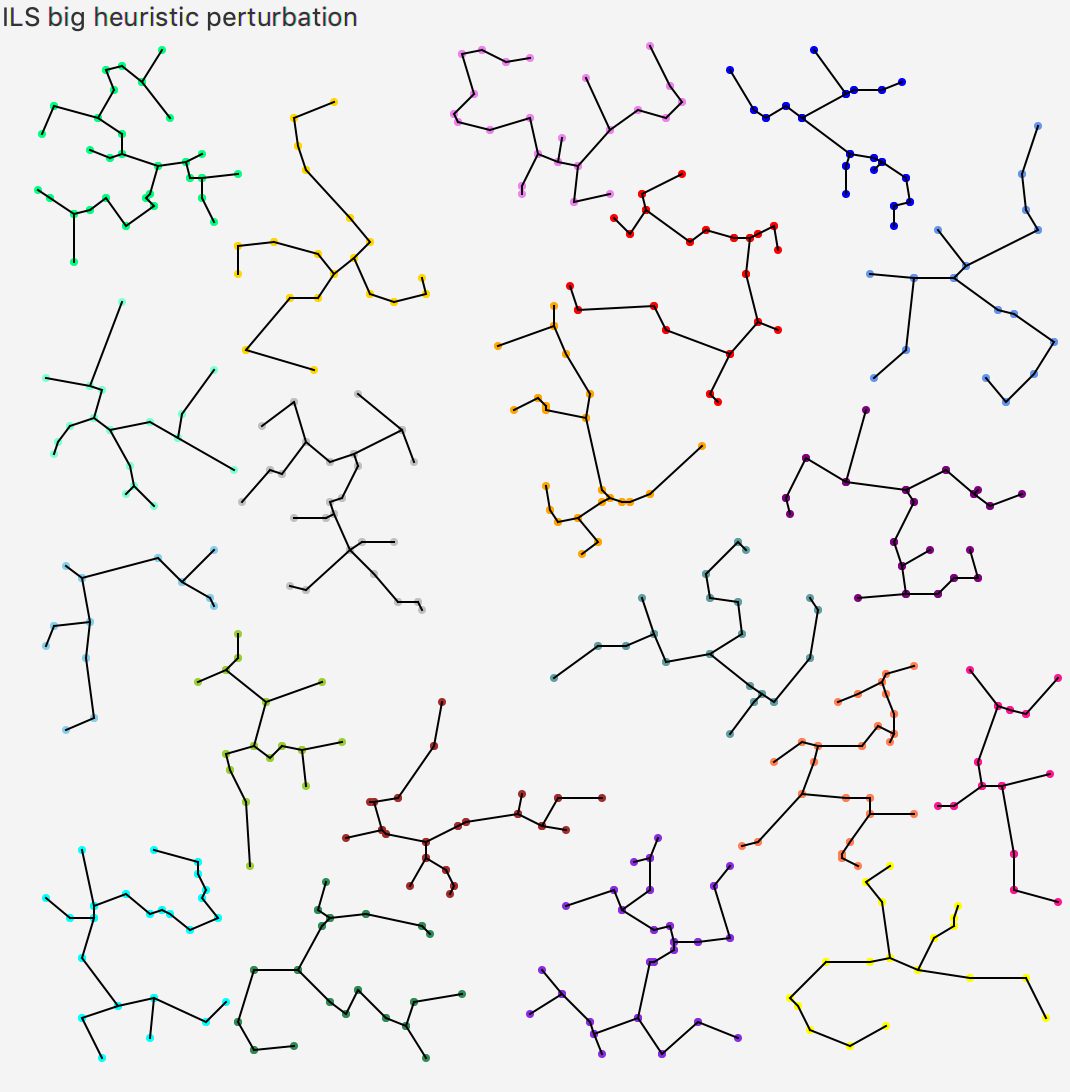
\includegraphics[width=0.45\textwidth]{sprawozdanie_4/ils_heuristic_mst.PNG}
        }
    \end{center}
    \caption{ILS big perturbation heuristic}
\end{figure}

\end{document}